% vim: textwidth=78 ai spell spelllang=en
\documentclass[11pt,a4paper]{article}

\usepackage[utf8x]{inputenc}
\usepackage[IL2]{fontenc}
\usepackage[final]{hyperref}
\usepackage{graphicx}
%\usepackage{multirow}
\usepackage{pdfpages}
\usepackage{xspace}
\usepackage[final]{listings}

\setlength{\textwidth}{140mm}
\setlength{\textheight}{220mm}
\setlength{\oddsidemargin}{12mm}

\font\logo fi-logo at 4cm

\setcounter{tocdepth}{2}

\lstset{tabsize=2,numbers=left,showstringspaces=false,breaklines=true,
        breakatwhitespace=true,escapeinside={(*@}{@*)},frame=l,
	basicstyle=\scriptsize}

\newcommand{\cdb}{\textsc{ClabureDB}\xspace}
\newcommand{\klee}{\textsc{Klee}\xspace}
\newcommand{\stan}{\textsc{Stanse}\xspace}
\newcommand{\symbio}{\textsc{Symbiotic}\xspace}

\begin{document}
\begin{titlepage}
\vspace{2cm}
\begin{center}
      {\sc Masaryk University\\Faculty of Informatics}

     \vspace{1cm}
     \logo SL

     \vspace{2cm}
     {\bf\huge Automatic Bug-finding Techniques for Linux Kernel}\\[0.8in]

     {\sc\large Dissertation Thesis}\\[0.4in]

     {\Large\bf Jiri Slaby}
     \vfill
     {\large Brno, autumn 2013}
     \vfill
\end{center}
     {\bf Supervisor:} prof. RNDr. Antonín Kučera, Ph.D.\\
     {\bf Supervisor-specialist:} doc. RNDr. Jan Strejček, PhD.\\[1cm]
     {\bf Supervisor's Signature: ......................}
\end{titlepage}

\pagestyle{plain}
\pagenumbering{roman}

\null\vfill
\section*{Acknowledgement}
I would like to thank my supervisors Prof. Kučera and Assoc. Prof.
Strejček for their patience with my ignorance. I thank my colleagues for their
ideas and inspiration. And of course my parents deserve many thanks for their
eternal support as well as Zuzanka does.

\newpage

\tableofcontents

\newpage
\pagenumbering{arabic}

\section{Introduction}

\subsection{Motivation}

Imprecise, useless tools for real use on a real SW.

\subsection{Current Techniques}

XYZ

Static Analysis

Abstract Interpretation

Symbolic Execution~\cite{king}

\subsection{The Goals}

\newpage
\section{Code Analysis}

\subsection{Static Analysis}
Abstract Interpretation~\cite{cousot}

\subsection{Symbolic Execution}
King~\cite{king}

\klee~\cite{klee} and clones.

\newpage
\section{Specifics of the Linux Kernel}
Are we going to tailor-make the thesis to the kernel?

Real code; self-contained code; call to be bug-free, otherwise
exploitable~\cite{exploit_vmsplice,exploit_proto_ops,exploit_tun}

\newpage
\section{Checking the Linux Kernel}
\stan~\cite{stanse}, projects like LDV (ISPRAS), Coverity~\cite{coverity}

\newpage
\section{Building Bug-database}
Necessity of a basis for improving static analyzers.

BSc thesis for web crawling (Ceľuch)

BSc thesis for web frontend (Hornák)

\stan output, SV-COMP~\cite{sv-comp} data

Implementing \cdb~\cite{claburedb}

\newpage
\section{Participating SV-COMP 2013}
Implementing inter-procedural LLVM slicer~\cite{llvm-slicer}, \symbio~\cite{symbiotic} and
participating~\cite{symbiotic-svcomp}.

\newpage
\section{Evaluation}
??

\newpage
\section{Related Work}

\newpage
\section{Conclusion}

\subsection{Contribution}

\subsection{Future Work}

\newpage
\bibliographystyle{plain}

\bibliography{dis}
\addcontentsline{toc}{section}{References}

\newpage
\appendix
\section{List of Publications}
\begin{itemize}
\item X
\item Y
\item Z
\end{itemize}
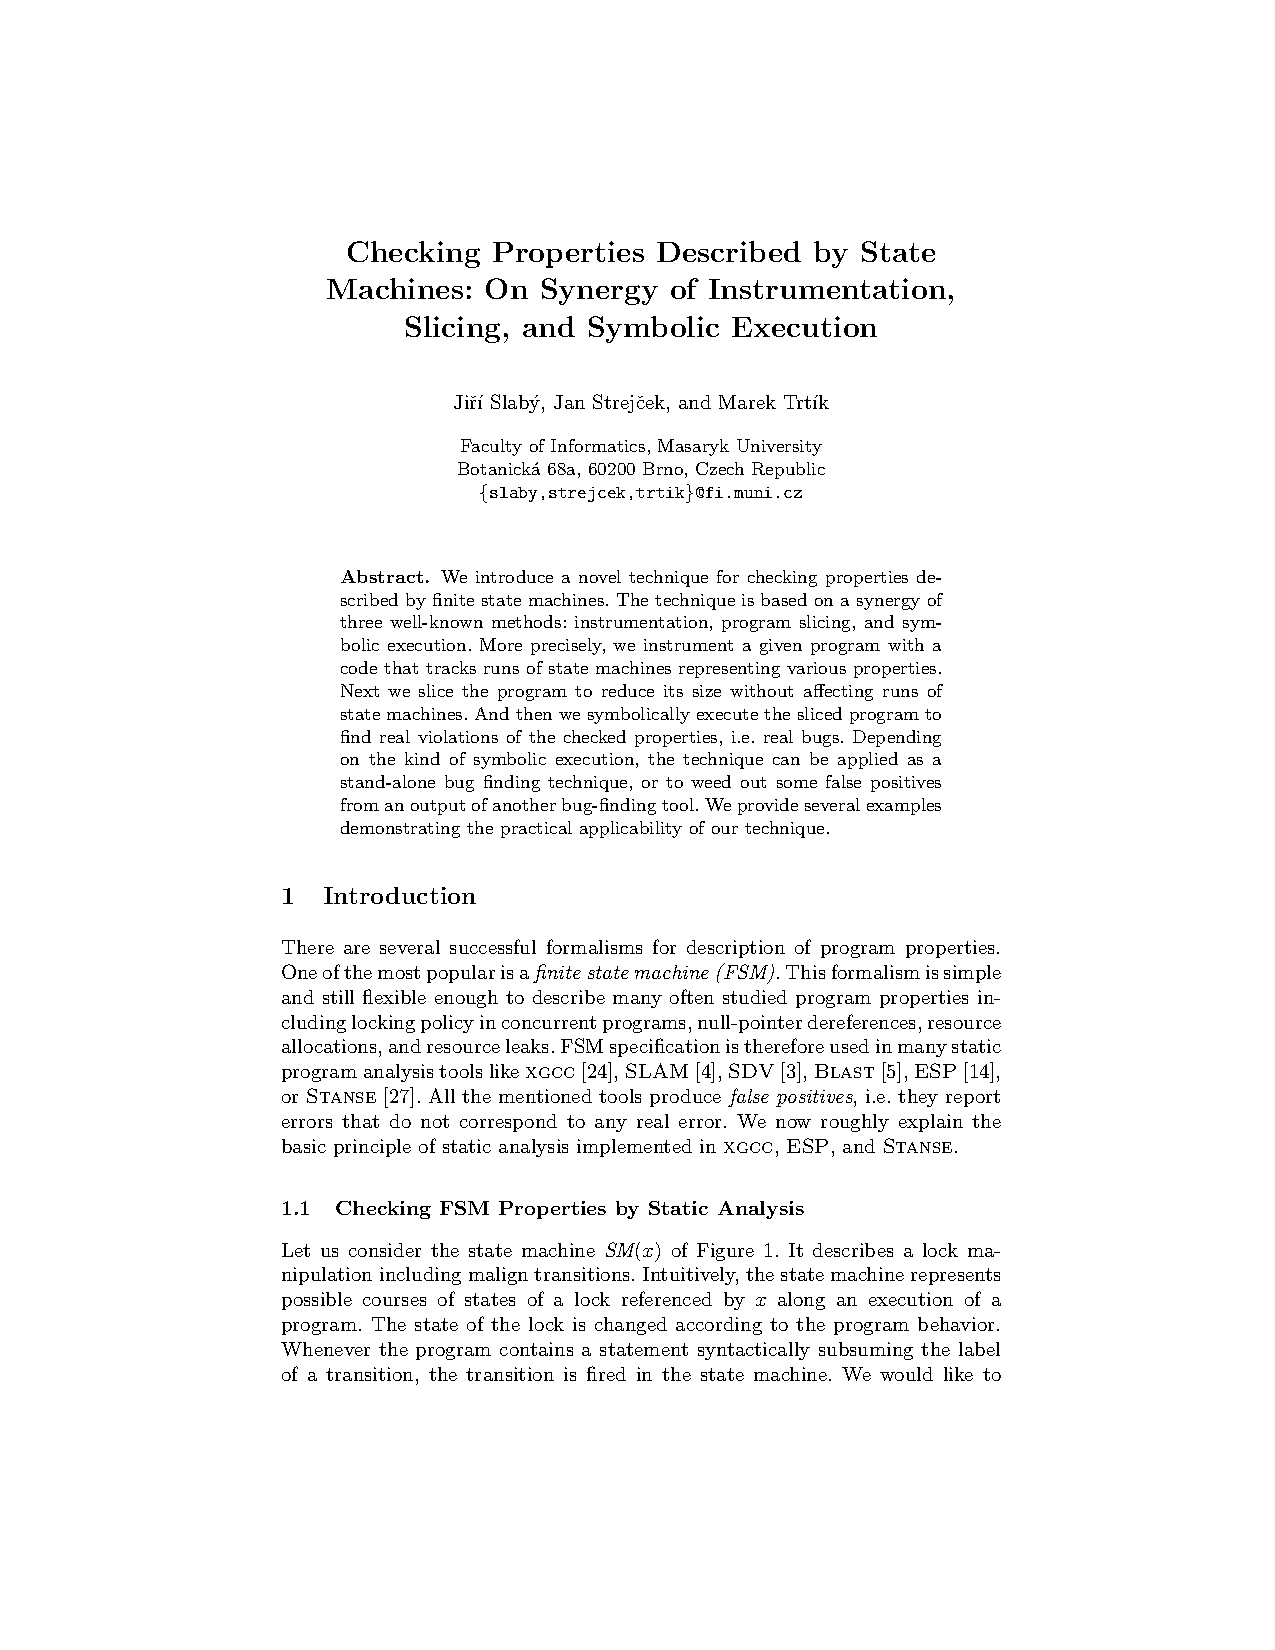
\includepdf[pages=-]{sse}
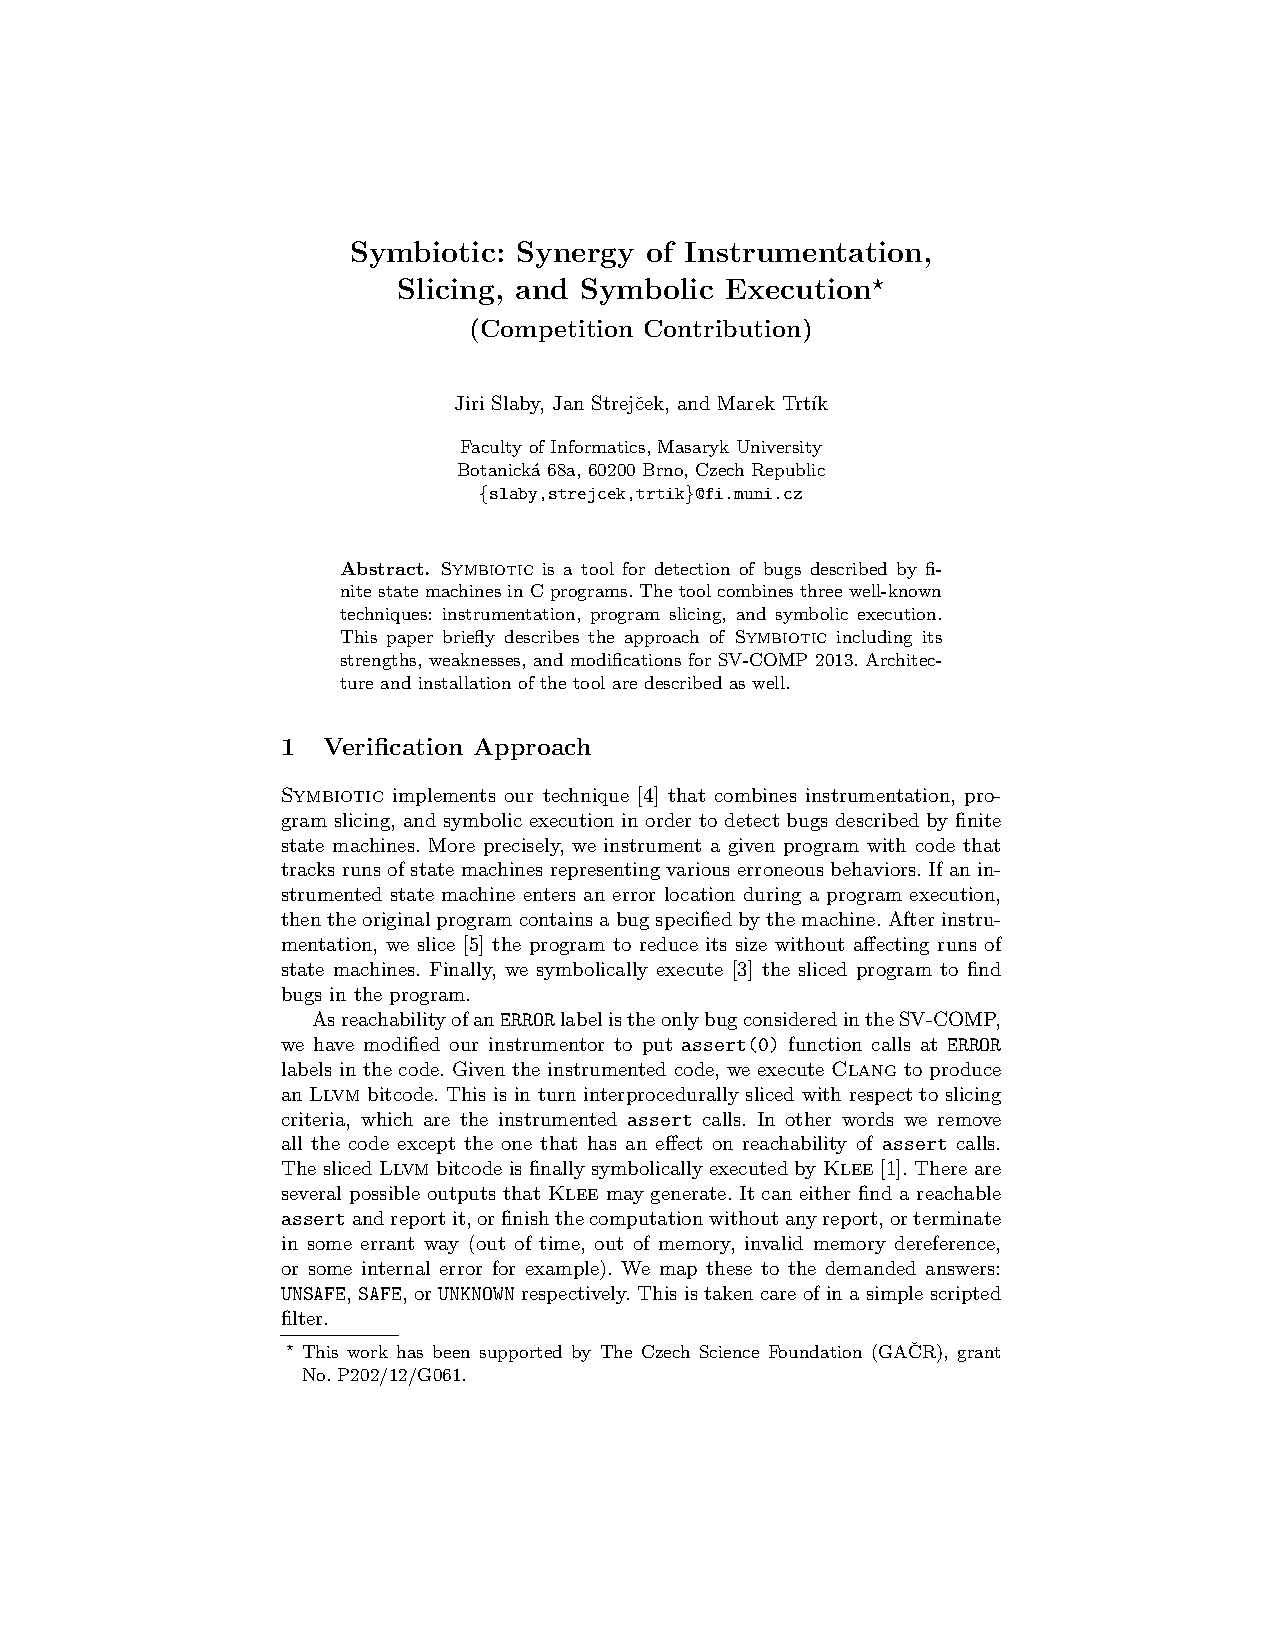
\includepdf[pages=-]{svcomp}
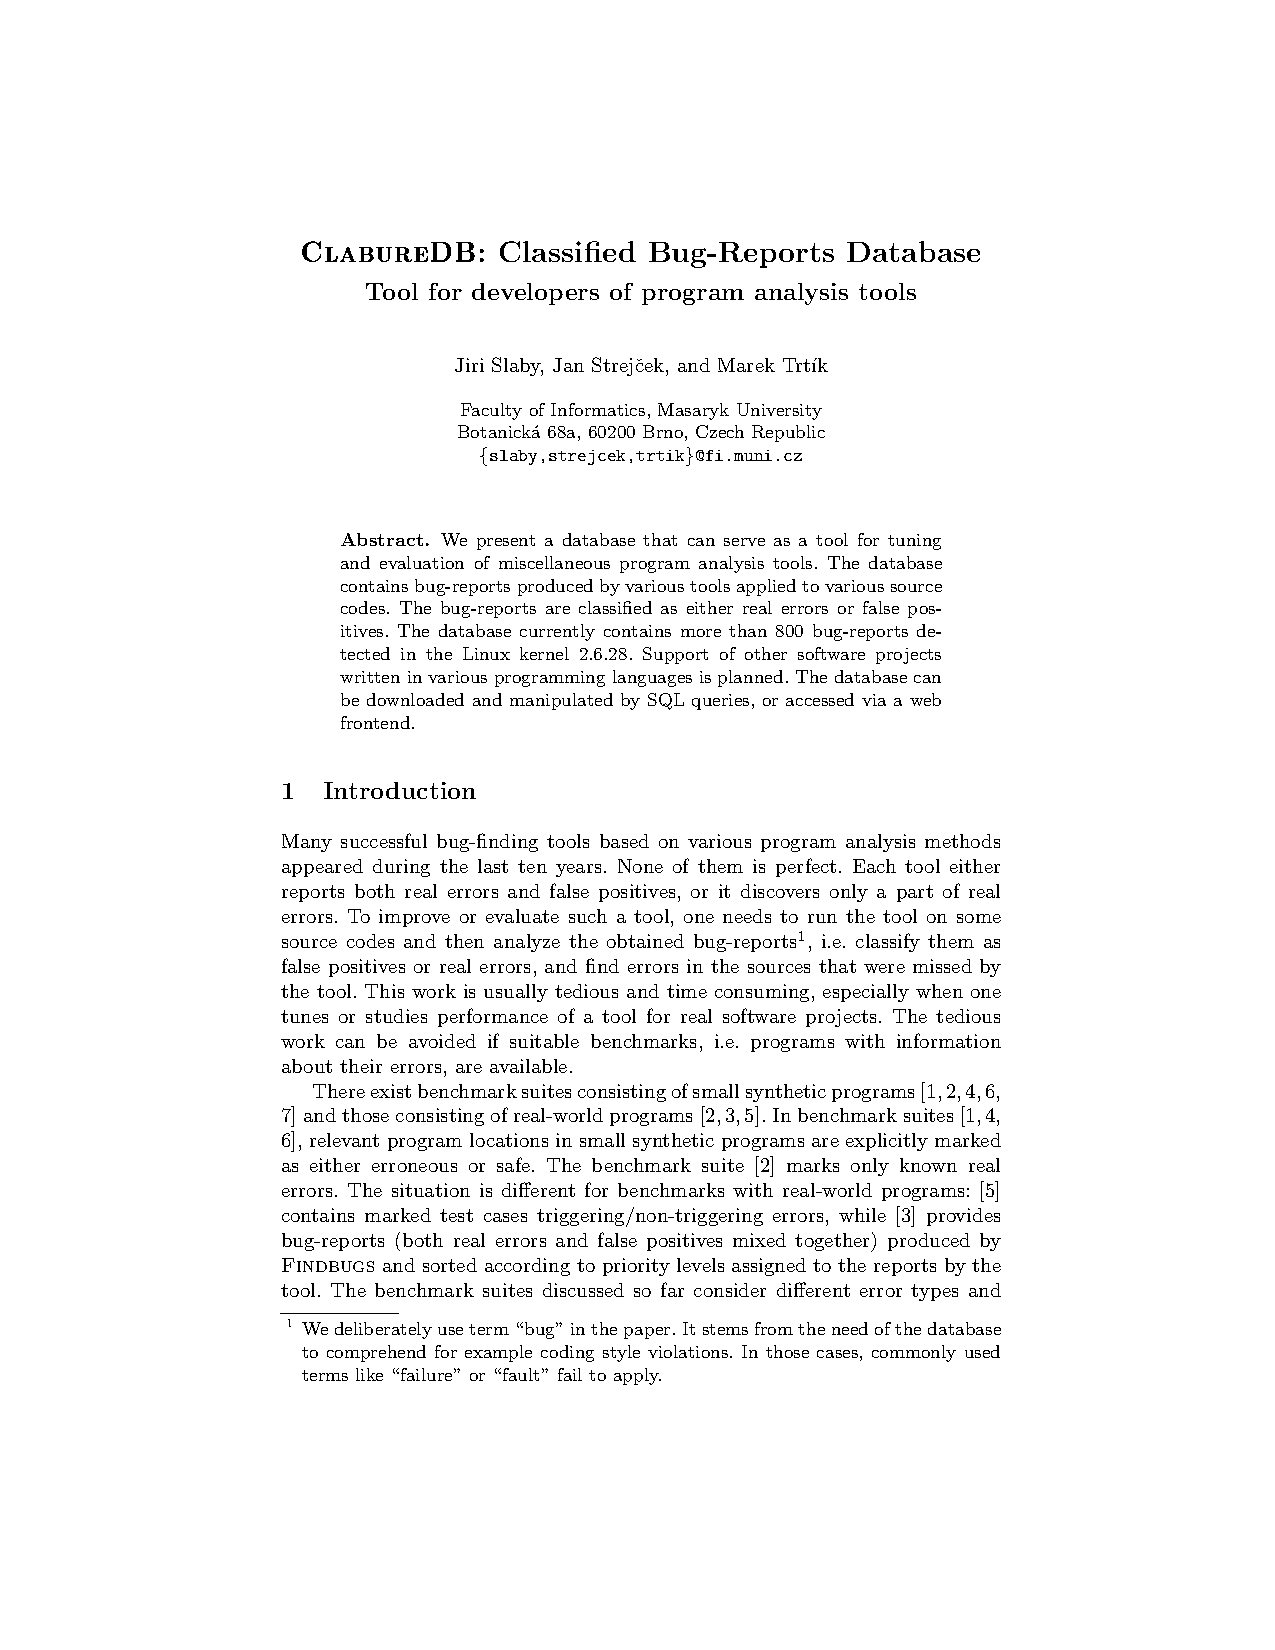
\includepdf[pages=-]{bd}

\end{document}
